%Traditional machine learning focuses on learning patterns from sets of (sometimes labelled) examples. 
%This is useful for learning approximations of concepts. % bad sentence
%However, for logical structures such as automata or propositional formulas, slight changes can result in very different behaviors. 
%It is not generally possible to exactly learn these structures from just labelled examples. 

Inductive synthesis or inductive learning 
is the synthesis of programs from examples or other observations. 
Most inductive synthesis follows the active learning model, where the
%Therefore, researchers have introduced the active learning model, where the
learner is allowed to make queries about the target concept to an oracle. 
Using the correct set of oracles can result in the polynomial time learnability of otherwise unlearnable sets \cite{angluin1988queries}. 
Recently, exact active learning has been applied to formal synthesis, where a program is automatically generated to fit a high-level specification \cite{jha2017theory}. 
This has been particularly useful in paradigms such as 
counter-example guided inductive synthesis \cite{solar2006combinatorial}.

Most exact learning algorithms for synthesis are monolithic, that is, even
if the concept (program) is made up of components, the algorithms seek to
learn the entire concept from interaction with an oracle.
In contrast, in this paper, we study the setting of modular concept learning,
where an exact-learning problem is analyzed by breaking it into independent components. 
If an element's membership in a concept depends solely on its membership in the components, learning the concept as a whole can be reduced to learning the components. 
We study concepts that are the Cartesian products (i.e., cross-products) of their component concepts.  
This can be thought of as learning conjunctions in that an element is part of a target concept if and only if its relevant variables are all of the component concepts. \todo{Is this clear? Should we be more explicit about the independent variable / concept class connection?}

We will focus on the oracle queries given in Table \ref{table:queries}.

\begin{table}
\label{table:queries}
\begin{center}
  \begin{tabularx}{\textwidth}{| c | c | c | X | }
    \hline
    Query Name & Symbol & Complexity & Oracle Definition \\ \hline
    Single Positive Query & $\oneposQ$ & $\oneposC(c)$ & Return a fixed $x \in c^*$ \\ \hline
    Positive Query & $\posQ$ & $\posC(c)$ & Return an $x\in c^*$ that has not yet been given as a positive example (if one exists)\\ \hline
    Membership Query & $\memQ$ & $\memC(c)$ & Given string $s$, return true iff $s \in c^*$ \\ \hline
    Equivalence Query & $\eqQ$ & $\eqC(c)$ & Given $c \in C$, return true if $c=c^*$ otherwise return $x \in (c \backslash c^*) \cup (c^* \backslash c)$\\ \hline 
    Subset Query & $\subQ$ & $\subC(c)$ & Given $c \in C$, return `true' if $c \subseteq c^*$ \mbox{  } otherwise return some $x \in c \backslash c^*$ \\ \hline
    Superset Query & $\supQ$ & $\supC(c)$ & Given $c \in C$, return `true' if $c \supseteq c^*$  otherwise return some $x \in c^* \backslash c$\\ \hline
    Example Query & $\pacQ_\dist$ & $\pacC(c, \dist)$ & Samples $x$ from $\dist$ and returns $x$ with a label indicating whether $x \in c^*$. \\ \hline
  \end{tabularx}
\end{center}
\caption{Types of queries studied in this paper.}
\end{table}

\subsection{A Motivating Example}

%\begin{figure}
%\centering
%\begin{varwidth}{\linewidth}
%\begin{lstlisting}
    %int x = ??;
    %int y = ??;
    %int a = f(x);
    %int b = g(y);
    %
    %$\Phi = \phi_1(a) \wedge \phi_2(b)$
%\end{lstlisting}
%\end{varwidth}
%\caption{A simple partial program to be synthesized to satisfy a specification $\Phi$}
%\label{sketch}
%\end{figure}

\begin{figure}[h]
\centering
%\subfloat[(a)]{
\begin{minipage}[b]{0.4 \textwidth}
%\begin{varwidth}{\linewidth}
\begin{lstlisting}
    int x = ??;
    int y = ??;
    int a = f(x);
    int b = g(y);
    
    $\Phi = \phi_1(a) \wedge \phi_2(b)$
\end{lstlisting}
\end{minipage}
%\label{sketch}}
%\end{varwidth}
\qquad
%\subfloat[(b)]{
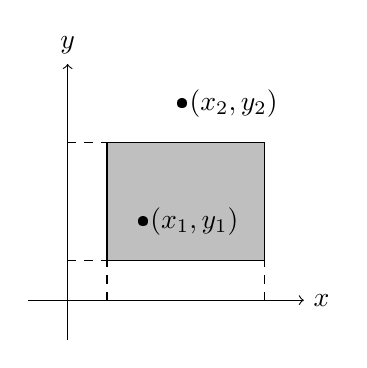
\begin{tikzpicture}
     \coordinate (BL) at (0.5,0.5);
     \coordinate (TR) at (2.5,2);
      \draw[->] (-0.5,0) -- (3,0) node[right] {$x$};
      \draw[->] (0,-0.5) -- (0,3) node[above] {$y$};
      \draw [draw=black] (BL) rectangle (TR);
      \filldraw [fill=lightgray, draw=black] (BL) rectangle (TR);
      \draw[dashed] (0,0.5) -- (BL);
      \draw[dashed] (0,2) -- (0.5,2);
      \draw[dashed] (0.5,0) -- (BL);
      \draw[dashed] (2.5,0) -- (2.5,0.5);
      \draw(.75,1) node[anchor = west]{\textbullet $(x_1,y_1)$};
      \draw(1.25,2.5) node[anchor = west]{\textbullet $(x_2,y_2)$};
      %\draw (1,1) node[draw=black, anchor=south] {.};
      %\tkzDefPoint(1,1){A};
      %\tkzLabelPoint[above](A){$(1,1)$};
\end{tikzpicture}
\caption{A simple partial program to be synthesized to satisfy a specification $\Phi$ (left) and the correct set of initial values for $x$ and $y$ (right).}
\label{sketch}
\label{sketchsolutions}
\end{figure}

To illustrate the learning problem, consider the sketching problem given in Figure \ref{sketch}.
Say we wanted to find the set of possible initial values for $x$ and $y$ that can replace the $??$ values so that the program satisfies $\Phi$.

Looking at the structure of this program and specification, we can see that the correctness of these two variables are independent of each other. 
Correct $x$ values are correct independent of $y$ and vice-versa.
Therefore, the set of settings will be the cross product of the acceptable settings for each variable.  
If an oracle can answer queries about correct $x$ or $y$ values separately, then the oracle can simply learn the acceptable values separately and take their Cartesian product. 

%\begin{figure}
%\begin{tikzpicture}
     %\coordinate (BL) at (0.5,0.5);
     %\coordinate (TR) at (2.5,2);
      %\draw[->] (-0.5,0) -- (3,0) node[right] {$x$};
      %\draw[->] (0,-0.5) -- (0,3) node[above] {$y$};
      %\draw [draw=black] (BL) rectangle (TR);
      %\filldraw [fill=lightgray, draw=black] (BL) rectangle (TR);
      %\draw[dashed] (0,0.5) -- (BL);
      %\draw[dashed] (0,2) -- (0.5,2);
      %\draw[dashed] (0.5,0) -- (BL);
      %\draw[dashed] (2.5,0) -- (2.5,0.5);
      %\draw(.75,1) node[anchor = west]{\textbullet $(x_1,y_1)$};
      %\draw(1.25,2.5) node[anchor = west]{\textbullet $(x_2,y_2)$};
      %%\draw (1,1) node[draw=black, anchor=south] {.};
      %%\tkzDefPoint(1,1){A};
      %%\tkzLabelPoint[above](A){$(1,1)$};
      %
%\end{tikzpicture}
%\caption{The correct set of initial values for $x$ and $y$.}
%\label{sketchsolutions}
%\end{figure}


If the correct values form intervals, the correct settings will look something like the rectangle shown in Figure \ref{sketchsolutions}.
An algorithm for learning this rectangle can try to simulate learning algorithms for each interval by acting as the oracle for each sublearner. 
For example, if both sublearners need a positive example, the learner can query the oracle for a positive example. 
Given the example $(x_1,y_1)$ as shown in the figure, the learner can then pass $x_1$ and $y_1$ to the sublearners as positive examples. 
However, this does not apply to negative examples, such as $(x_2, y_2)$ in the figure. 
In this example, $x_2$ is in its target interval, but $y_2$ is not. 
The learner has no way of knowing which subconcept a negative element fails on.
Handling negative counterexamples is one of the main challenges of this paper.




